\section{Results}
\label{sec:results}

The main claim survives every cell it was tested in: training-free per-layer logit-lens uncertainty statistics are class-separable hallucination scores at intermediate depth in all six model $\times$ dataset cells (selection-split corrected AUROC 0.6092--0.7011 against a 0.55 gate), and the best screened intermediate layer beats the same sweep's final-layer entropy readout in every cell. We present the existence grid first, then the structure inside it: the dataset dependence of the depth advantage, the signal-family pattern, the anchor forensics that determined what counts as a baseline, and one finding that contradicted our own prediction. Every number below is a selection-split point estimate from a single seed; none is held-out performance.

\subsection{The existence grid}
\label{sec:existence-grid}

Table~\ref{tab:existence-grid} reports the six selected tuples with their within-sweep final-layer baselines. Figure~\ref{fig:gate-grid} shows the headline comparison --- per-cell best-intermediate AUROC against the 0.55 gate and the final-layer bar; every intermediate bar clears both.

\begin{table*}[t]
\centering
\caption{Selection-split corrected AUROC per cell (single seed, no CIs). Depth margin = best intermediate $-$ within-sweep final-layer entropy.}
\label{tab:existence-grid}
\begin{tabular}{llccc}
\toprule
Cell & Selected (layer, signal) & Intermediate AUROC & Final-layer entropy AUROC & Depth margin \\
\midrule
LLaMA-2 / TriviaQA & L31, adj.\ KL & 0.6522 & 0.5928 & +0.059 \\
LLaMA-2 / TruthfulQA & L29, entropy & 0.7011 & 0.6669 & +0.034 \\
Mistral / TriviaQA & L31, max-prob & 0.6092 & 0.5447 & +0.064 \\
Mistral / TruthfulQA & L31, adj.\ KL & 0.6570 & 0.6048 & +0.052 \\
LLaMA-3 / TriviaQA & L28, entropy & 0.6868 & 0.5566 & +0.130 \\
LLaMA-3 / TruthfulQA & L31, max-prob & 0.6213 & 0.6178 & +0.0035 \\
\bottomrule
\end{tabular}
\end{table*}

\begin{figure*}[t]
\centering
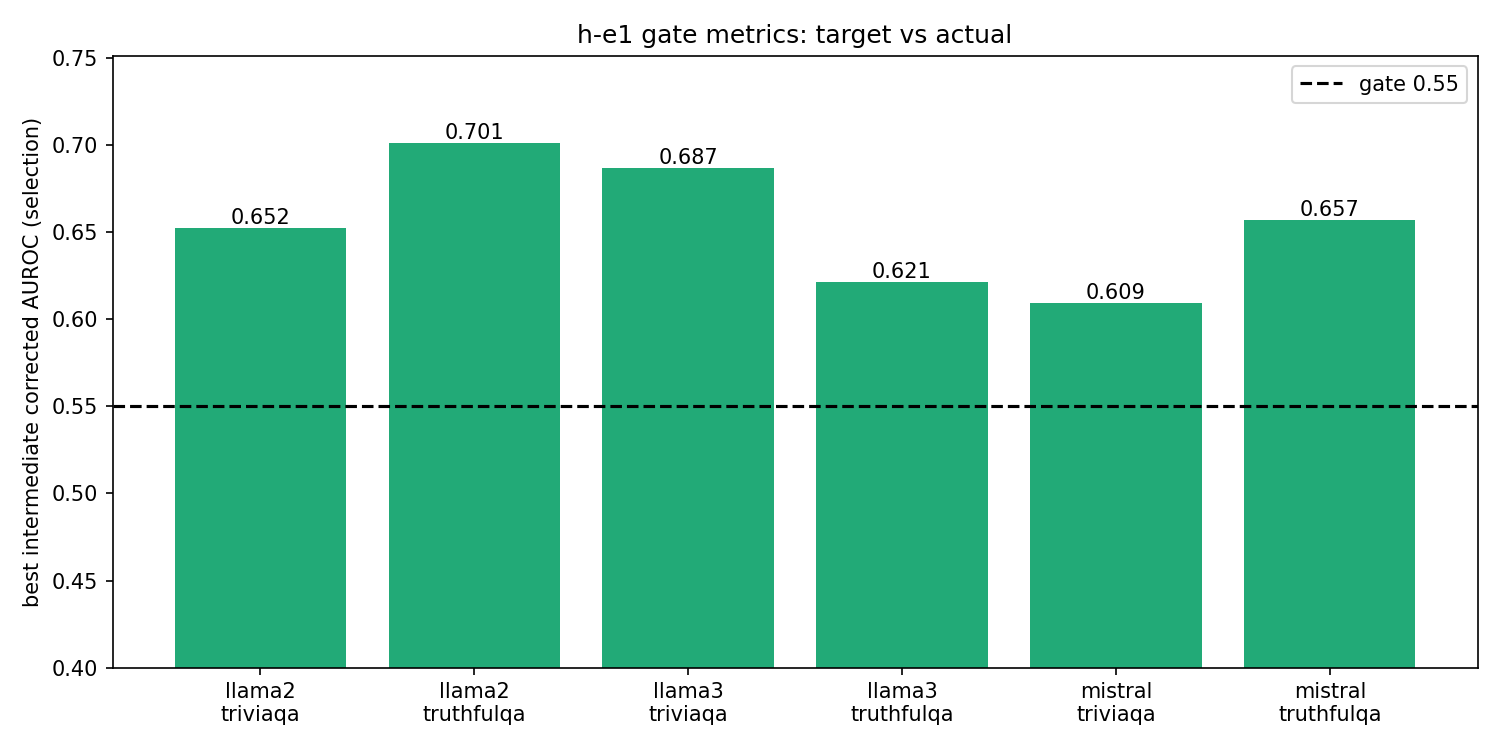
\includegraphics[width=0.9\textwidth]{figures/gate_metrics_bar.png}
\caption{Existence gate grid --- per-cell best intermediate corrected AUROC vs. the 0.55 gate and the within-sweep final-layer entropy baseline, all six cells.}
\label{fig:gate-grid}
\end{figure*}

The answer to RQ1 is yes, everywhere: the gate clears by +0.059 (Mistral/TriviaQA) to +0.151 (LLaMA-2/TruthfulQA). These are point estimates --- we computed no confidence intervals and make no distributional claim about the margins; we note only, as a point-estimate comparison, that the thinnest gate margin is an order of magnitude larger than the thinnest depth margin of Section~\ref{sec:depth-advantage}. The so-what is universality within scope: the signal appears in a base LLaMA, a base Mistral, and an RLHF-tuned LLaMA-3, under two different labeling protocols --- the intermediate-over-final consensus does extend to statistics that need no probe, at least at existence tier. The selected layers also concentrate: every winner sits at L28--L31, four of six at L31 itself --- the informative surface is the late-but-not-last band just before output calibration. Figure~\ref{fig:auroc-heatmap} shows the full layer $\times$ signal grid; the late-band concentration is visible in every cell, not an artifact of the argmax.

\begin{figure*}[t]
\centering
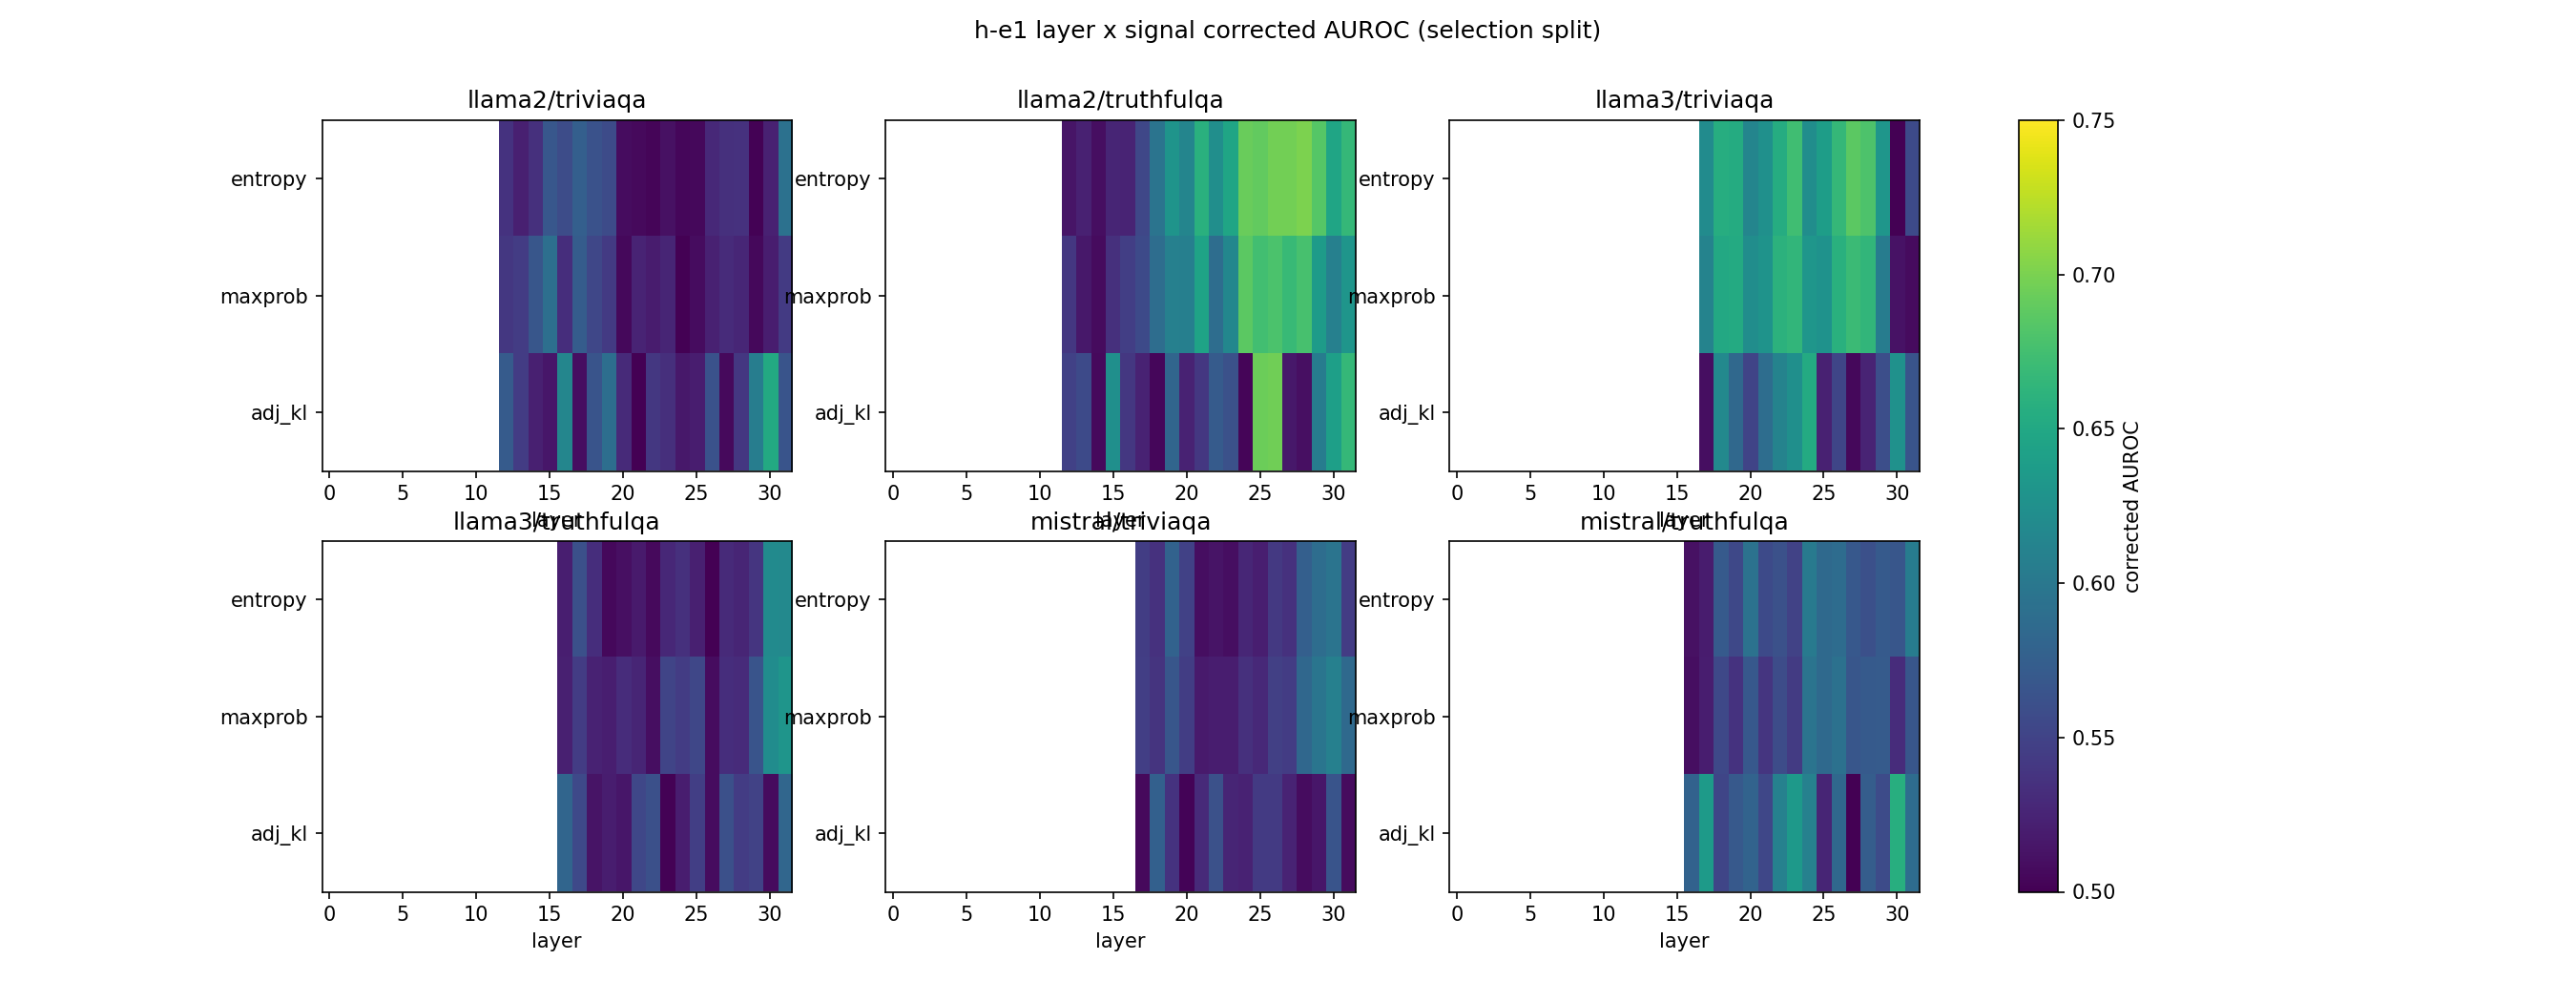
\includegraphics[width=0.9\textwidth]{figures/auroc_heatmap.png}
\caption{Corrected AUROC across screened layers and signals for all six cells. Informative depth concentrates at L28--L31.}
\label{fig:auroc-heatmap}
\end{figure*}

\subsection{The depth advantage is universal in direction, dataset-dependent in size}
\label{sec:depth-advantage}

RQ2 also resolves 6/6: the best screened intermediate layer beats the within-sweep final-layer entropy readout in every cell. But the margins split cleanly by dataset. On TriviaQA they are substantial --- +0.059, +0.064, +0.130 --- while on TruthfulQA they thin to +0.034, +0.052, and +0.0035, because TruthfulQA final layers are already strong (entropy AUROC 0.6048--0.6669). We flag the thinnest cell plainly: at +0.0035 on 408 selection examples with no confidence interval, LLaMA-3/TruthfulQA's depth advantage is within plausible noise, and we count it as direction-consistent rather than as evidence. The claim degrades gracefully --- five of six margins exceed 0.03 --- but ``6/6'' is a point-estimate statement, not a statistical one.

The interpretation is a nuance the mechanism story needs: depth helps most where the final layer is weakest. Where output calibration leaves little separation at L32 (TriviaQA, final-layer AUROC 0.54--0.59), reading before calibration recovers a lot; where the final layer already separates classes (TruthfulQA), there is less to recover. This is consistent with the calibration-suppression reading --- suppression as relative attenuation, not destruction --- while bounding it: whatever suppresses the signal is dataset-dependent. Whether that reflects TruthfulQA's adversarial question design, its similarity-based label protocol, or small-sample variance cannot be decided from this grid; all three explanations remain live.

\subsection{Signal families: belief revision as a detection score}
\label{sec:signal-families}

Adjacent-layer KL --- a statistic with no detection-time precedent, previously used only to steer decoding --- is the best signal in two of six cells, with entropy and max-probability each also best in two: an even three-way split. Its strongest showing is the LLaMA-2/TriviaQA cell (Figure~\ref{fig:kl-showcase}), where the top three intermediate scores are all adj.\ KL: L31 at 0.6522, L17 at 0.6145, L30 at 0.6062. That the winning signal differs across datasets within every model --- and the winning layer within two of the three --- also vindicates selecting the full (layer, signal, direction) tuple per cell rather than fixing any element a priori.

\begin{figure}[t]
\centering
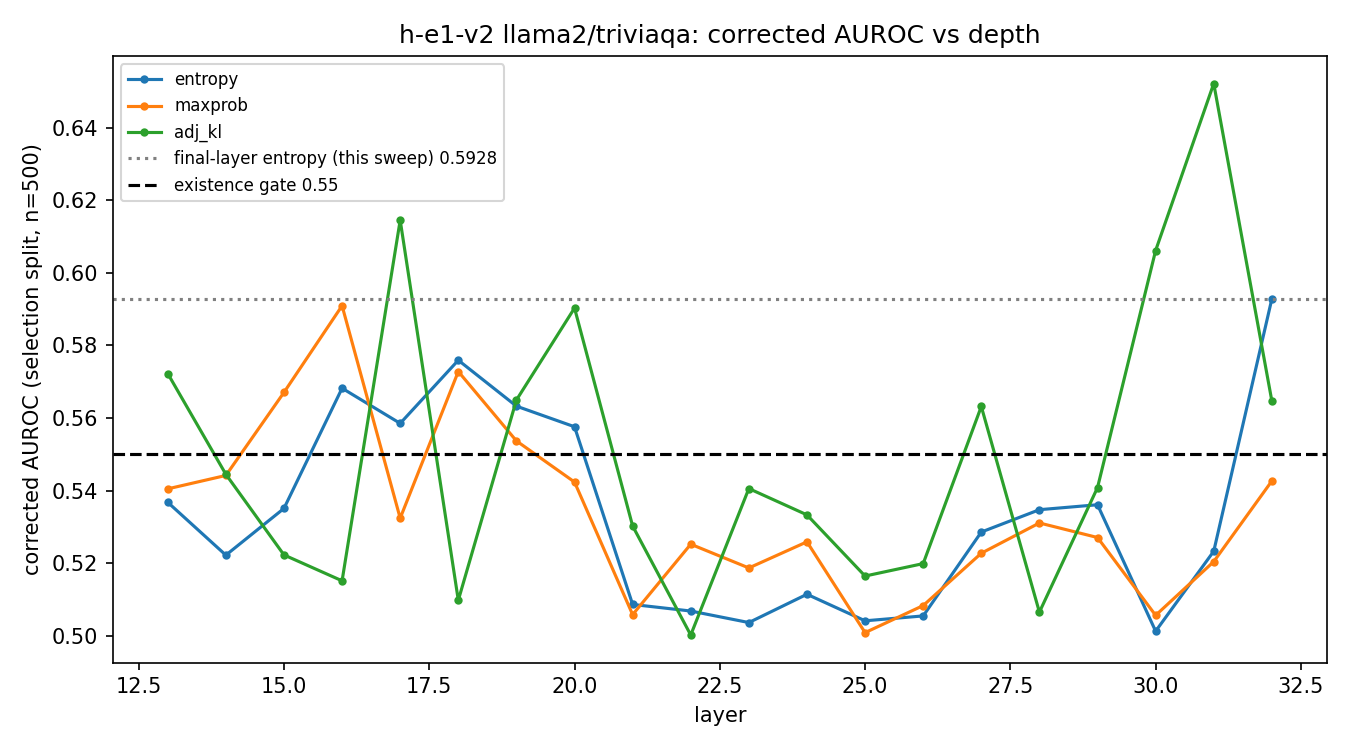
\includegraphics[width=\columnwidth]{figures/auroc_vs_depth_llama2_triviaqa.png}
\caption{AUROC vs. depth for LLaMA-2/TriviaQA --- the three signal curves with the 0.55 gate and final-layer baseline. The top three intermediate scores are all adjacent-layer KL.}
\label{fig:kl-showcase}
\end{figure}

The so-what: inter-layer belief revision is a first-class detection signal, not just a decoding heuristic --- to our knowledge the first detection-time use of this quantity, and the paper's most novel single observation. What adj.\ KL at L31 \emph{measures}, however, is genuinely undecidable from our data. Two readings fit: it is an independent ``turbulence'' signal --- persistent belief revision as a distinct facet of unresolved competition --- or it is a meter on the calibration step itself, scoring how much the last layers rewrite the distribution. Both are calibration-adjacent; separating them needs the fusion test and the correlation analysis staged as future work, both computable from the published caches with zero GPU.

\subsection{Anchor forensics: what happened to the baseline this study set out to beat}
\label{sec:forensics}

This study was designed around a documented failure: the archived motivating record (Section~\ref{sec:intro}) put final-layer entropy at AUROC 0.5186 on LLaMA-2/TriviaQA. The v1 experiment gated on reproducing that number within $\pm$0.03 --- and the halt gate fired 47 seconds into what was budgeted as a $\sim$2.5-hour GPU campaign. The observed value was 0.5928 on the selection split (0.5739 on the full set), a deviation of +0.0742 against a 0.03 tolerance. A provenance audit found the reference protocol differed in six documented ways: random-sample vs. first-slice data selection, bare vs. templated prompt, substring vs. normalized-alias labels, generation-time vs. teacher-forced lens entropy, bfloat16 vs. fp16, and full-set vs. selection-split evaluation. The anchor was unsatisfiable by construction --- no correct implementation could close a gap created by measuring a different thing. Figure~\ref{fig:anchor-breach} shows the breach against the tolerance band. The redesigned protocol-internal anchor (Section~\ref{sec:anchor}) then passed all five clauses on the full v2 sweep with zero spurious halts; the descriptive cross-run check found direction consistent with the motivating record in 4/6 cells, both inconsistencies on cells that record never code-verified.

\begin{figure*}[t]
\centering
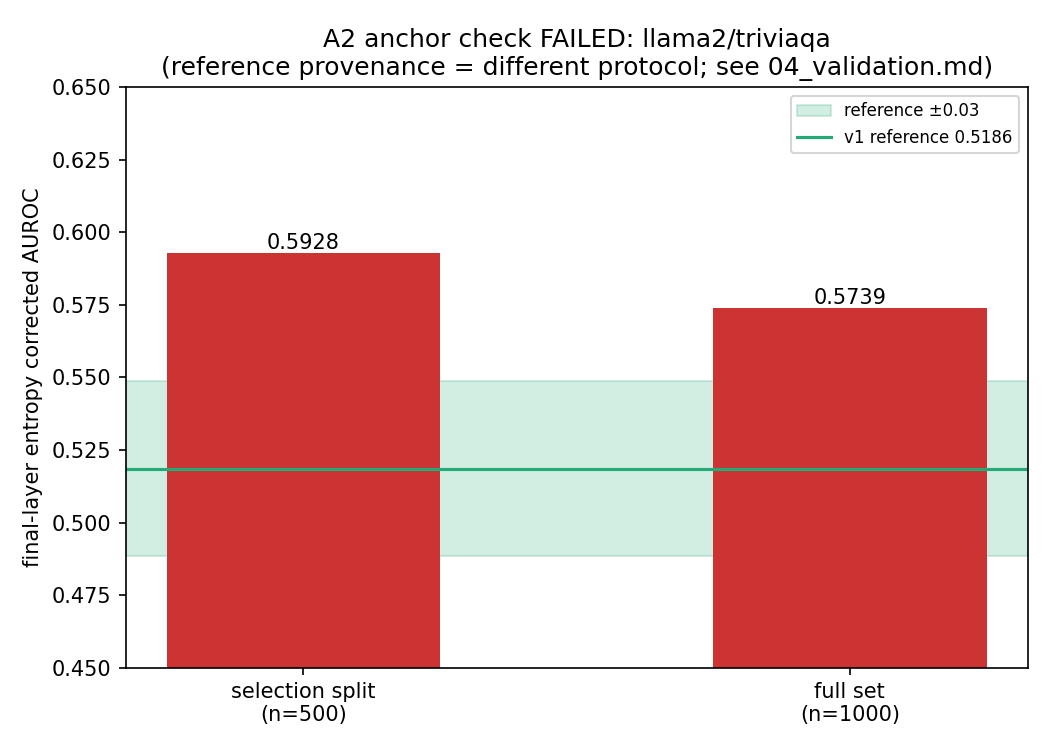
\includegraphics[width=0.9\textwidth]{figures/h-e1_anchor_check_llama2_triviaqa.png}
\caption{The v1 anchor breach --- observed final-layer entropy AUROC vs. the cross-protocol reference and its $\pm$0.03 tolerance band on LLaMA-2/TriviaQA.}
\label{fig:anchor-breach}
\end{figure*}

We report this as a result, not an incident report. The so-what is twofold. Scientifically: AUROC magnitudes for weak uncertainty signals are protocol-bound --- six ordinary protocol choices moved the same cell by +0.074 --- so direction transfers across protocols but magnitude does not, and any comparison this paper makes is within-sweep for that reason. Practically: a cheap designed halt gate converted a doomed campaign into a 47-second diagnosis, which is the strongest argument we can offer for building validity gates into evaluation pipelines before spending compute.

\subsection{A prediction reversed: the depth advantage does not track tuning status as hypothesized}
\label{sec:prediction-reversed}

Our mechanism draft predicted that base LLaMA-2, presumed worst-suppressed, would gain most from depth readout, and instruct-tuned LLaMA-3 least. The data reverse this ordering: the largest TriviaQA depth margin (+0.130, Figure~\ref{fig:llama3-margin}) belongs to LLaMA-3-8B-Instruct --- the model predicted to need depth least --- with Mistral (+0.064) and LLaMA-2 (+0.059) behind it. A revised hypothesis fits: instruct tuning may \emph{sharpen} final-layer calibration, strengthening suppression rather than weakening it --- still a calibration story, with the opposite tuning polarity. We state this descriptively only and verify nothing: with a single instruct model in the grid, tuning status is confounded with everything else about the checkpoint, and the base-vs-instruct pair study that could decide it is future work.

\begin{figure}[t]
\centering
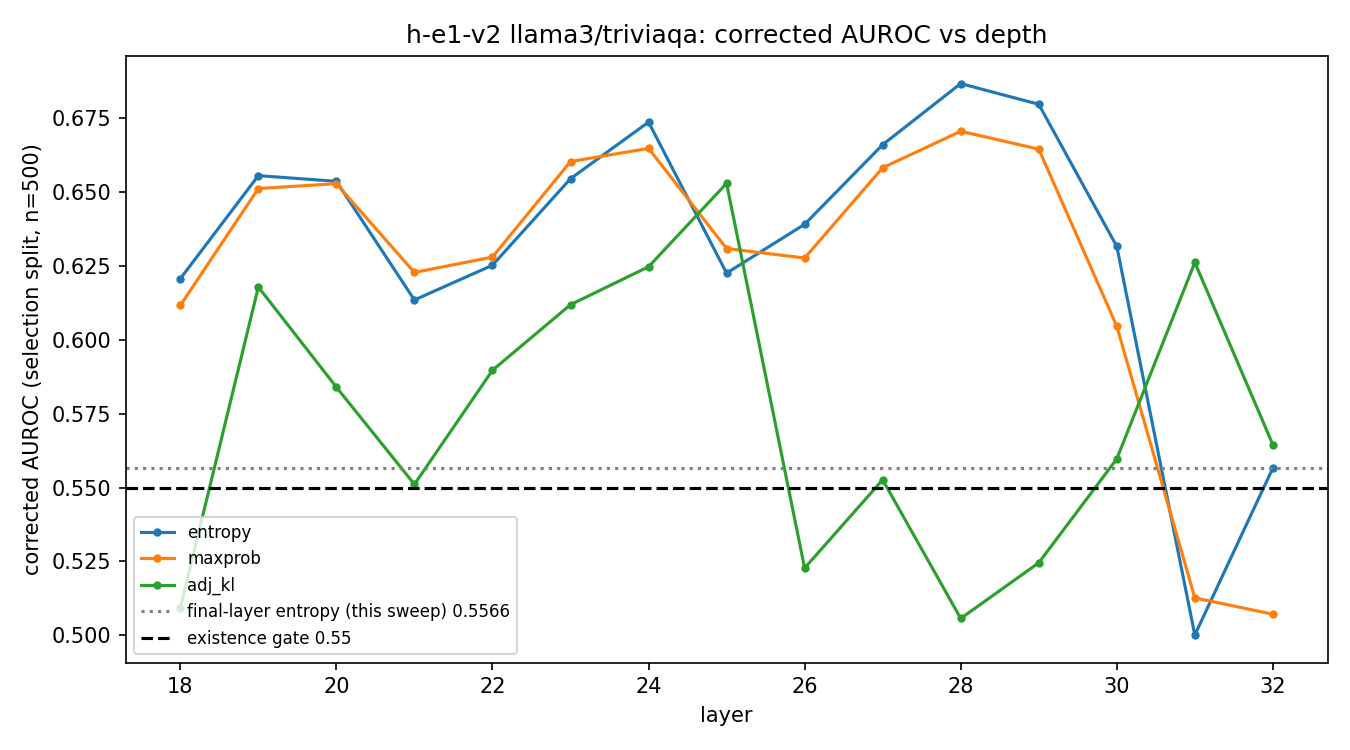
\includegraphics[width=\columnwidth]{figures/auroc_vs_depth_llama3_triviaqa.png}
\caption{AUROC vs. depth for LLaMA-3/TriviaQA --- the largest depth margin in the grid (+0.130), on the model predicted to need depth least.}
\label{fig:llama3-margin}
\end{figure}
